\chapter{Descrizione generale}

\section{Inquadramento}
La piattaforma è stata progettata con lo scopo di erogare dei servizi tipicamente richiesti in ambito aziendale come la gestione delle
informazioni degli utenti, meccanismi di autenticazioni e autorizzazione, l'invio di
email e la sottoscrizione a servizi generici in versione di prova.
L'erogazione di questi servizi avviene grazie ai seguenti elementi (vedi Figura \ref{fig:Piattaforma}):
\begin{itemize}
    \itemsep0em
    \item Client: applicazione front-end che permette agli utenti di sfruttare le funzionalità della piattaforma inviando delle richieste alla API e mostrando le risposte.
    \item API Web: web Server che permette di gestire le richieste del client e fornisce una interfaccia REST per erogare i servizi.
    \item Microservizio Mailer: servizio interno che gestisce la generazione dei template delle email e l'invio.
    \item Message Broker: permette di fare interagire API Web e il microservizio Mailer.
    \item Email System: sistema esterno utilizzato per l'effettivo invio delle email agli utenti.
    \item Database: permette di gestire i dati in modo permanente.
\end{itemize}

\begin{figure}[H]
    \centering
    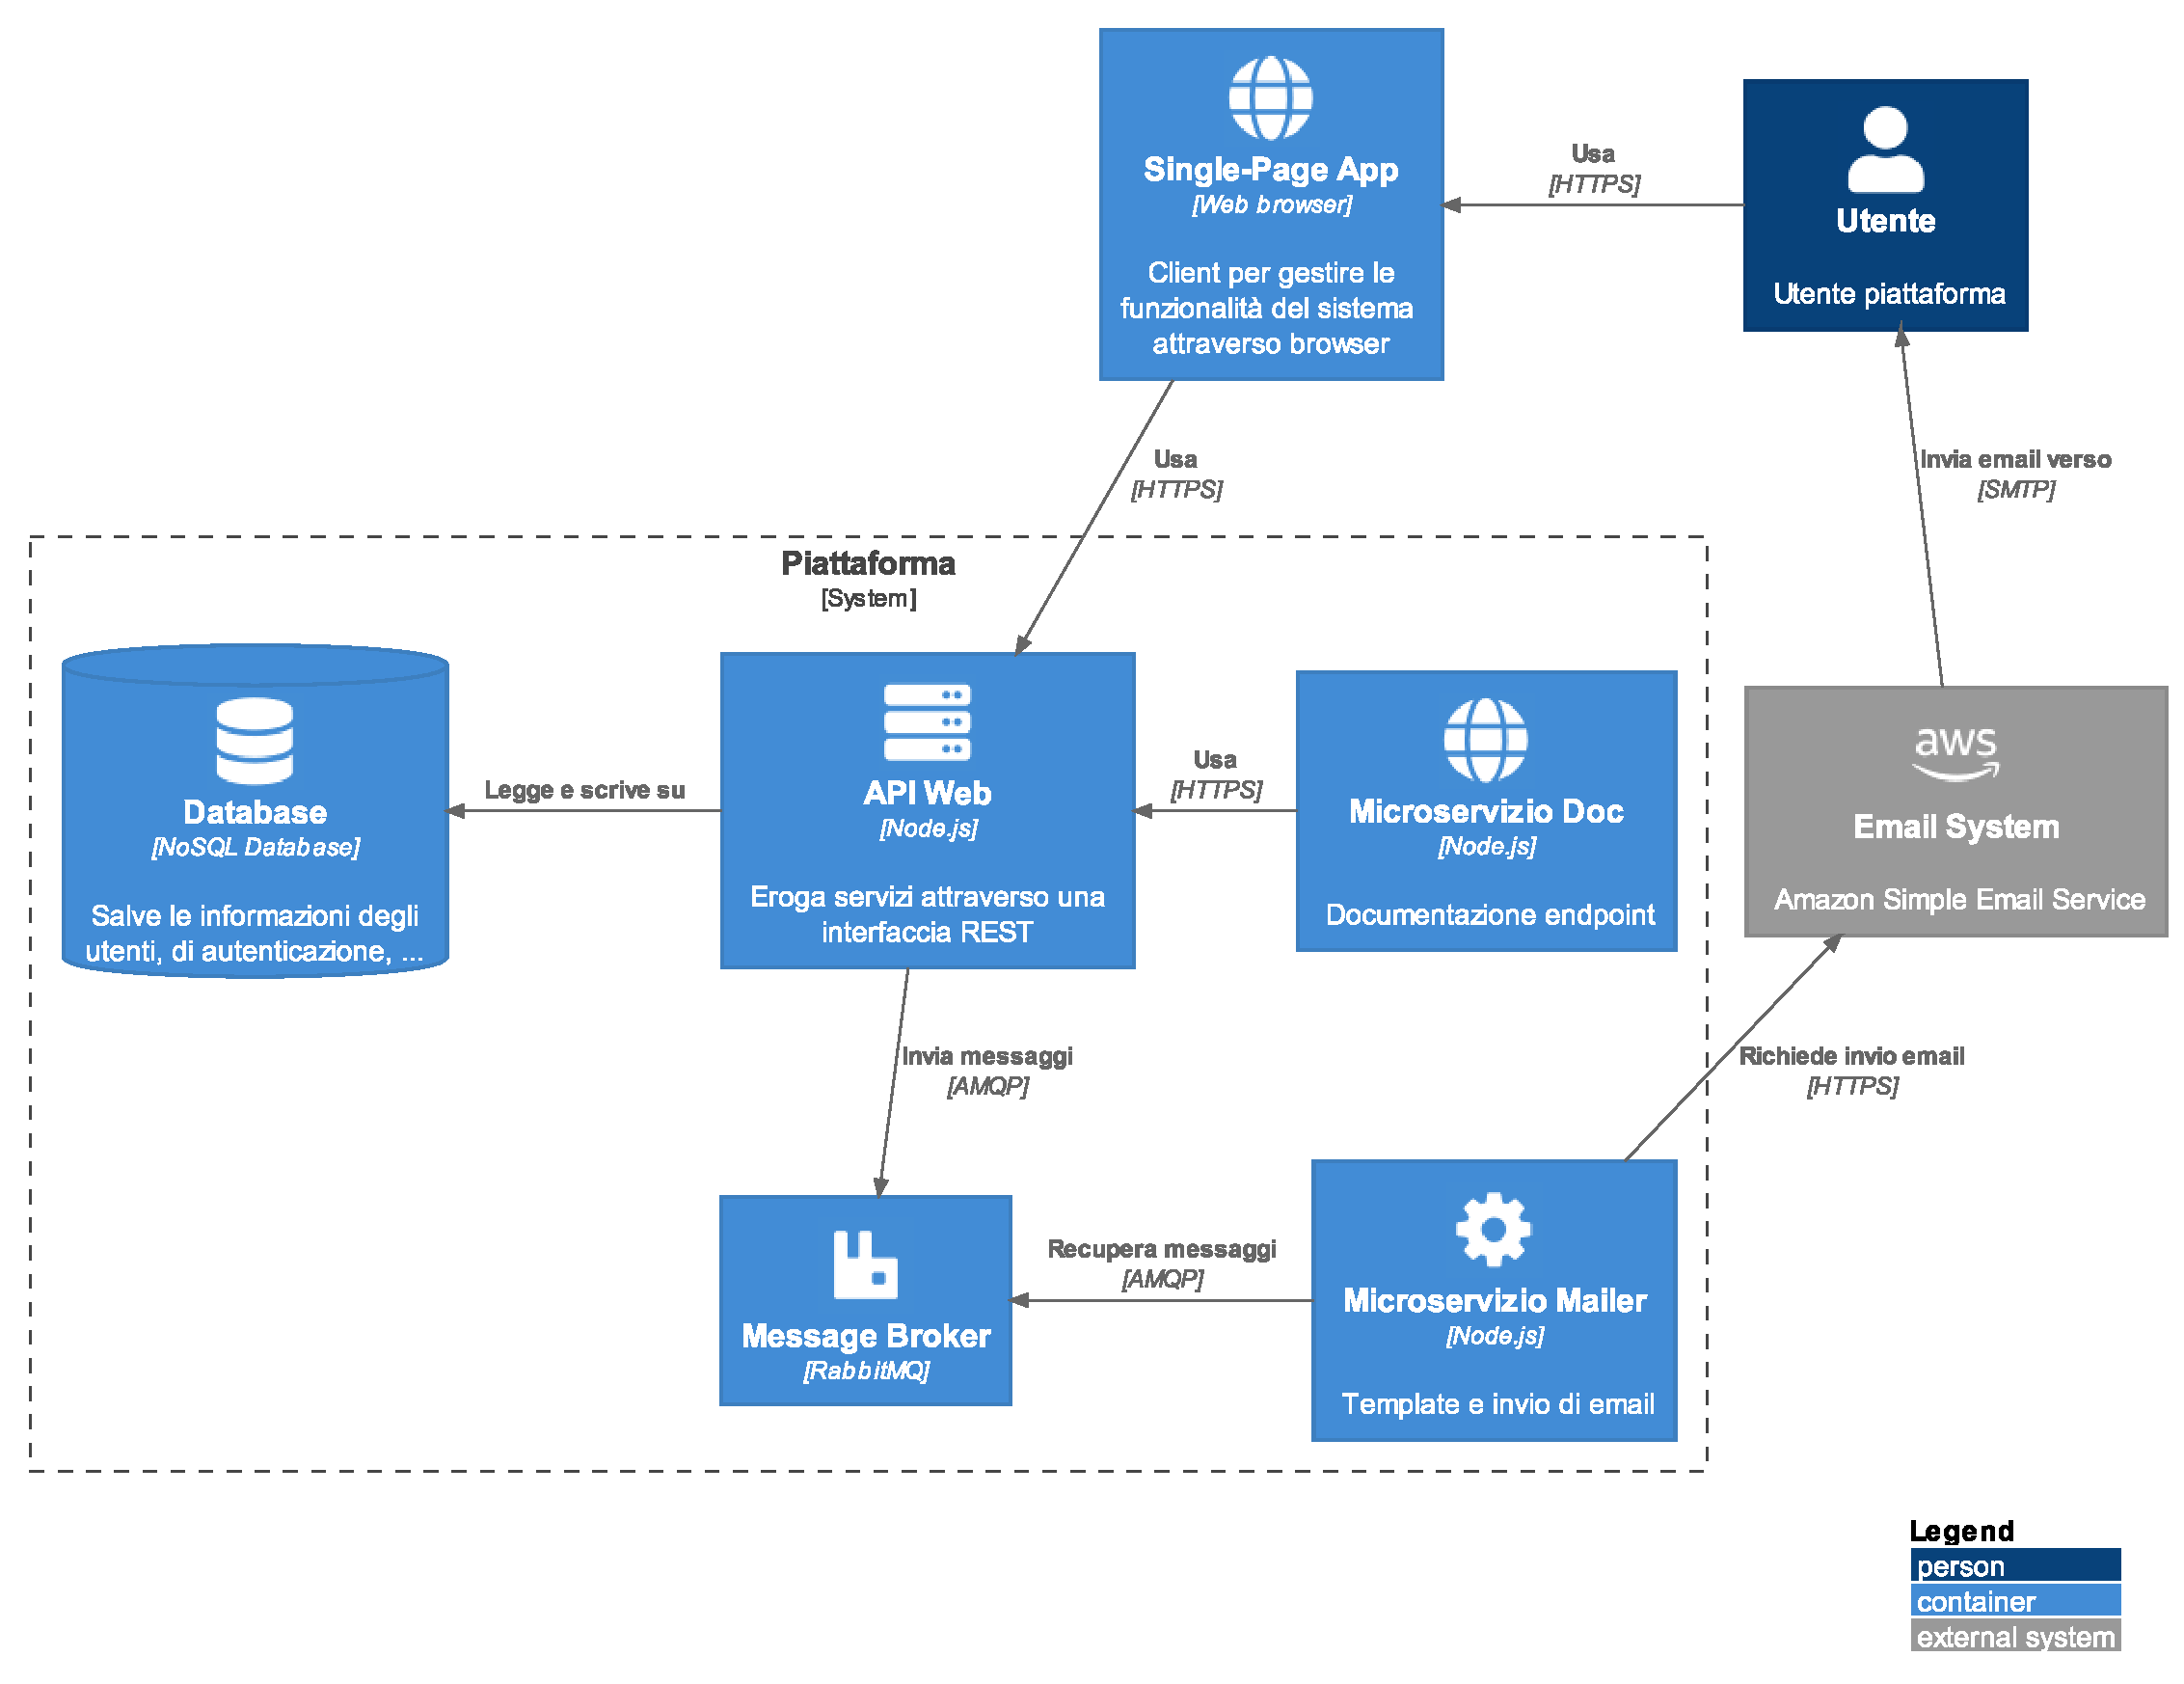
\includegraphics[width=0.8\textwidth]{container-diagram-generale.eps}
    \caption{Architettura piattaforma}
    \label{fig:Piattaforma}
\end{figure}
\newpage

\section{Vincoli generali}
Scalabilità
robustezza
sicurezza
collaborazione


\section{Metodologia di lavoro}
La metodologia di lavoro adottata per la realizzazione della piattaforma si ispira alla metodologia agile e alle pratiche di DevOps.

La metodologia agile è un modello di sviluppo finalizzato a rilasciare frequentemente software funzionante e di qualità al cliente.
Annunciato ufficialmente nel 2001 attravero il Manifesto Agile questo modello si basa sui seguenti principi:
\begin{itemize}
    \itemsep0em
    \item 
\end{itemize}
Emerge quindi in modo evidente la contrapposizione con i classici modelli di sviluppo come il modello a cascata.
Infatti qui si hanno blablabla che si contrappongono con vlablabla

questa metofologia agile permette quindi questi benefici
1 2 3 4 5 

con queste accortezze (Svantaggi)

